
%% bare_jrnl.tex
%% V1.4b
%% 2015/08/26
%% by Michael Shell
%% see http://www.michaelshell.org/
%% for current contact information.
%%
%% This is a skeleton file demonstrating the use of IEEEtran.cls
%% (requires IEEEtran.cls version 1.8b or later) with an IEEE
%% journal paper.
%%
%% Support sites:
%% http://www.michaelshell.org/tex/ieeetran/
%% http://www.ctan.org/pkg/ieeetran
%% and
%% http://www.ieee.org/

%%*************************************************************************
%% Legal Notice:
%% This code is offered as-is without any warranty either expressed or
%% implied; without even the implied warranty of MERCHANTABILITY or
%% FITNESS FOR A PARTICULAR PURPOSE! 
%% User assumes all risk.
%% In no event shall the IEEE or any contributor to this code be liable for
%% any damages or losses, including, but not limited to, incidental,
%% consequential, or any other damages, resulting from the use or misuse
%% of any information contained here.
%%
%% All comments are the opinions of their respective authors and are not
%% necessarily endorsed by the IEEE.
%%
%% This work is distributed under the LaTeX Project Public License (LPPL)
%% ( http://www.latex-project.org/ ) version 1.3, and may be freely used,
%% distributed and modified. A copy of the LPPL, version 1.3, is included
%% in the base LaTeX documentation of all distributions of LaTeX released
%% 2003/12/01 or later.
%% Retain all contribution notices and credits.
%% ** Modified files should be clearly indicated as such, including  **
%% ** renaming them and changing author support contact information. **
%%*************************************************************************


% *** Authors should verify (and, if needed, correct) their LaTeX system  ***
% *** with the testflow diagnostic prior to trusting their LaTeX platform ***
% *** with production work. The IEEE's font choices and paper sizes can   ***
% *** trigger bugs that do not appear when using other class files.       ***                          ***
% The testflow support page is at:
% http://www.michaelshell.org/tex/testflow/



\documentclass[final,journal,10pt,letterpaper,oneside,twocolumn,compsoc]%
{IEEEtran}
%
% If IEEEtran.cls has not been installed into the LaTeX system files,
% manually specify the path to it like:
% \documentclass[journal]{../sty/IEEEtran}





% Some very useful LaTeX packages include:
% (uncomment the ones you want to load)


% *** MISC UTILITY PACKAGES ***
%
%\usepackage{ifpdf}
% Heiko Oberdiek's ifpdf.sty is very useful if you need conditional
% compilation based on whether the output is pdf or dvi.
% usage:
% \ifpdf
%   % pdf code
% \else
%   % dvi code
% \fi
% The latest version of ifpdf.sty can be obtained from:
% http://www.ctan.org/pkg/ifpdf
% Also, note that IEEEtran.cls V1.7 and later provides a builtin
% \ifCLASSINFOpdf conditional that works the same way.
% When switching from latex to pdflatex and vice-versa, the compiler may
% have to be run twice to clear warning/error messages.






% *** CITATION PACKAGES ***
%
\usepackage{cite}
% cite.sty was written by Donald Arseneau
% V1.6 and later of IEEEtran pre-defines the format of the cite.sty package
% \cite{} output to follow that of the IEEE. Loading the cite package will
% result in citation numbers being automatically sorted and properly
% "compressed/ranged". e.g., [1], [9], [2], [7], [5], [6] without using
% cite.sty will become [1], [2], [5]--[7], [9] using cite.sty. cite.sty's
% \cite will automatically add leading space, if needed. Use cite.sty's
% noadjust option (cite.sty V3.8 and later) if you want to turn this off
% such as if a citation ever needs to be enclosed in parenthesis.
% cite.sty is already installed on most LaTeX systems. Be sure and use
% version 5.0 (2009-03-20) and later if using hyperref.sty.
% The latest version can be obtained at:
% http://www.ctan.org/pkg/cite
% The documentation is contained in the cite.sty file itself.






% *** GRAPHICS RELATED PACKAGES ***
%
\ifCLASSINFOpdf
   \usepackage[pdftex]{graphicx}
  % declare the path(s) where your graphic files are
   \graphicspath{ {graphics/} }%{{../pdf/}{../jpeg/}}
  % and their extensions so you won't have to specify these with
  % every instance of \includegraphics
   \DeclareGraphicsExtensions{.pdf}
\else
  % or other class option (dvipsone, dvipdf, if not using dvips). graphicx
  % will default to the driver specified in the system graphics.cfg if no
  % driver is specified.
  % \usepackage[dvips]{graphicx}
  % declare the path(s) where your graphic files are
  % \graphicspath{{../eps/}}
  % and their extensions so you won't have to specify these with
  % every instance of \includegraphics
  % \DeclareGraphicsExtensions{.eps}
\fi
% graphicx was written by David Carlisle and Sebastian Rahtz. It is
% required if you want graphics, photos, etc. graphicx.sty is already
% installed on most LaTeX systems. The latest version and documentation
% can be obtained at: 
% http://www.ctan.org/pkg/graphicx
% Another good source of documentation is "Using Imported Graphics in
% LaTeX2e" by Keith Reckdahl which can be found at:
% http://www.ctan.org/pkg/epslatex
%
% latex, and pdflatex in dvi mode, support graphics in encapsulated
% postscript (.eps) format. pdflatex in pdf mode supports graphics
% in .pdf, .jpeg, .png and .mps (metapost) formats. Users should ensure
% that all non-photo figures use a vector format (.eps, .pdf, .mps) and
% not a bitmapped formats (.jpeg, .png). The IEEE frowns on bitmapped formats
% which can result in "jaggedy"/blurry rendering of lines and letters as
% well as large increases in file sizes.
%
% You can find documentation about the pdfTeX application at:
% http://www.tug.org/applications/pdftex





% *** MATH PACKAGES ***
%
\usepackage{amsmath}
% A popular package from the American Mathematical Society that provides
% many useful and powerful commands for dealing with mathematics.
%
% Note that the amsmath package sets \interdisplaylinepenalty to 10000
% thus preventing page breaks from occurring within multiline equations. Use:
%\interdisplaylinepenalty=2500
% after loading amsmath to restore such page breaks as IEEEtran.cls normally
% does. amsmath.sty is already installed on most LaTeX systems. The latest
% version and documentation can be obtained at:
% http://www.ctan.org/pkg/amsmath





% *** SPECIALIZED LIST PACKAGES ***
%
%\usepackage{algorithmic}
% algorithmic.sty was written by Peter Williams and Rogerio Brito.
% This package provides an algorithmic environment fo describing algorithms.
% You can use the algorithmic environment in-text or within a figure
% environment to provide for a floating algorithm. Do NOT use the algorithm
% floating environment provided by algorithm.sty (by the same authors) or
% algorithm2e.sty (by Christophe Fiorio) as the IEEE does not use dedicated
% algorithm float types and packages that provide these will not provide
% correct IEEE style captions. The latest version and documentation of
% algorithmic.sty can be obtained at:
% http://www.ctan.org/pkg/algorithms
% Also of interest may be the (relatively newer and more customizable)
% algorithmicx.sty package by Szasz Janos:
% http://www.ctan.org/pkg/algorithmicx




% *** ALIGNMENT PACKAGES ***
%
%\usepackage{array}
% Frank Mittelbach's and David Carlisle's array.sty patches and improves
% the standard LaTeX2e array and tabular environments to provide better
% appearance and additional user controls. As the default LaTeX2e table
% generation code is lacking to the point of almost being broken with
% respect to the quality of the end results, all users are strongly
% advised to use an enhanced (at the very least that provided by array.sty)
% set of table tools. array.sty is already installed on most systems. The
% latest version and documentation can be obtained at:
% http://www.ctan.org/pkg/array


% IEEEtran contains the IEEEeqnarray family of commands that can be used to
% generate multiline equations as well as matrices, tables, etc., of high
% quality.




% *** SUBFIGURE PACKAGES ***
%\ifCLASSOPTIONcompsoc
%  \usepackage[caption=false,font=normalsize,labelfont=sf,textfont=sf]{subfig}
%\else
%  \usepackage[caption=false,font=footnotesize]{subfig}
%\fi
% subfig.sty, written by Steven Douglas Cochran, is the modern replacement
% for subfigure.sty, the latter of which is no longer maintained and is
% incompatible with some LaTeX packages including fixltx2e. However,
% subfig.sty requires and automatically loads Axel Sommerfeldt's caption.sty
% which will override IEEEtran.cls' handling of captions and this will result
% in non-IEEE style figure/table captions. To prevent this problem, be sure
% and invoke subfig.sty's "caption=false" package option (available since
% subfig.sty version 1.3, 2005/06/28) as this is will preserve IEEEtran.cls
% handling of captions.
% Note that the Computer Society format requires a larger sans serif font
% than the serif footnote size font used in traditional IEEE formatting
% and thus the need to invoke different subfig.sty package options depending
% on whether compsoc mode has been enabled.
%
% The latest version and documentation of subfig.sty can be obtained at:
% http://www.ctan.org/pkg/subfig




% *** FLOAT PACKAGES ***
%
%\usepackage{fixltx2e}
% fixltx2e, the successor to the earlier fix2col.sty, was written by
% Frank Mittelbach and David Carlisle. This package corrects a few problems
% in the LaTeX2e kernel, the most notable of which is that in current
% LaTeX2e releases, the ordering of single and double column floats is not
% guaranteed to be preserved. Thus, an unpatched LaTeX2e can allow a
% single column figure to be placed prior to an earlier double column
% figure.
% Be aware that LaTeX2e kernels dated 2015 and later have fixltx2e.sty's
% corrections already built into the system in which case a warning will
% be issued if an attempt is made to load fixltx2e.sty as it is no longer
% needed.
% The latest version and documentation can be found at:
% http://www.ctan.org/pkg/fixltx2e


\usepackage{stfloats}
% stfloats.sty was written by Sigitas Tolusis. This package gives LaTeX2e
% the ability to do double column floats at the bottom of the page as well
% as the top. (e.g., "\begin{figure*}[!b]" is not normally possible in
% LaTeX2e). It also provides a command:
%\fnbelowfloat
% to enable the placement of footnotes below bottom floats (the standard
% LaTeX2e kernel puts them above bottom floats). This is an invasive package
% which rewrites many portions of the LaTeX2e float routines. It may not work
% with other packages that modify the LaTeX2e float routines. The latest
% version and documentation can be obtained at:
% http://www.ctan.org/pkg/stfloats
% Do not use the stfloats baselinefloat ability as the IEEE does not allow
% \baselineskip to stretch. Authors submitting work to the IEEE should note
% that the IEEE rarely uses double column equations and that authors should try
% to avoid such use. Do not be tempted to use the cuted.sty or midfloat.sty
% packages (also by Sigitas Tolusis) as the IEEE does not format its papers in
% such ways.
% Do not attempt to use stfloats with fixltx2e as they are incompatible.
% Instead, use Morten Hogholm'a dblfloatfix which combines the features
% of both fixltx2e and stfloats:
%
% \usepackage{dblfloatfix}
% The latest version can be found at:
% http://www.ctan.org/pkg/dblfloatfix




%\ifCLASSOPTIONcaptionsoff
%  \usepackage[nomarkers]{endfloat}
% \let\MYoriglatexcaption\caption
% \renewcommand{\caption}[2][\relax]{\MYoriglatexcaption[#2]{#2}}
%\fi
% endfloat.sty was written by James Darrell McCauley, Jeff Goldberg and 
% Axel Sommerfeldt. This package may be useful when used in conjunction with 
% IEEEtran.cls'  captionsoff option. Some IEEE journals/societies require that
% submissions have lists of figures/tables at the end of the paper and that
% figures/tables without any captions are placed on a page by themselves at
% the end of the document. If needed, the draftcls IEEEtran class option or
% \CLASSINPUTbaselinestretch interface can be used to increase the line
% spacing as well. Be sure and use the nomarkers option of endfloat to
% prevent endfloat from "marking" where the figures would have been placed
% in the text. The two hack lines of code above are a slight modification of
% that suggested by in the endfloat docs (section 8.4.1) to ensure that
% the full captions always appear in the list of figures/tables - even if
% the user used the short optional argument of \caption[]{}.
% IEEE papers do not typically make use of \caption[]'s optional argument,
% so this should not be an issue. A similar trick can be used to disable
% captions of packages such as subfig.sty that lack options to turn off
% the subcaptions:
% For subfig.sty:
% \let\MYorigsubfloat\subfloat
% \renewcommand{\subfloat}[2][\relax]{\MYorigsubfloat[]{#2}}
% However, the above trick will not work if both optional arguments of
% the \subfloat command are used. Furthermore, there needs to be a
% description of each subfigure *somewhere* and endfloat does not add
% subfigure captions to its list of figures. Thus, the best approach is to
% avoid the use of subfigure captions (many IEEE journals avoid them anyway)
% and instead reference/explain all the subfigures within the main caption.
% The latest version of endfloat.sty and its documentation can obtained at:
% http://www.ctan.org/pkg/endfloat
%
% The IEEEtran \ifCLASSOPTIONcaptionsoff conditional can also be used
% later in the document, say, to conditionally put the References on a 
% page by themselves.




% *** PDF, URL AND HYPERLINK PACKAGES ***
%
\usepackage{url}
% url.sty was written by Donald Arseneau. It provides better support for
% handling and breaking URLs. url.sty is already installed on most LaTeX
% systems. The latest version and documentation can be obtained at:
% http://www.ctan.org/pkg/url
% Basically, \url{my_url_here}.




% *** Do not adjust lengths that control margins, column widths, etc. ***
% *** Do not use packages that alter fonts (such as pslatex).         ***
% There should be no need to do such things with IEEEtran.cls V1.6 and later.
% (Unless specifically asked to do so by the journal or conference you plan
% to submit to, of course. )


% correct bad hyphenation here
\hyphenation{op-tical net-works semi-conduc-tor}


\begin{document}
\bstctlcite{IEEEexample:BSTcontrol}
%
% paper title
% Titles are generally capitalized except for words such as a, an, and, as,
% at, but, by, for, in, nor, of, on, or, the, to and up, which are usually
% not capitalized unless they are the first or last word of the title.
% Linebreaks \\ can be used within to get better formatting as desired.
% Do not put math or special symbols in the title.
\title{Weighting Environmental Impacts in Software Distribution Systems}
%
%
% author names and IEEE memberships
% note positions of commas and nonbreaking spaces ( ~ ) LaTeX will not break
% a structure at a ~ so this keeps an author's name from being broken across
% two lines.
% use \thanks{} to gain access to the first footnote area
% a separate \thanks must be used for each paragraph as LaTeX2e's \thanks
% was not built to handle multiple paragraphs
%

\author{Bertrand~Ithurburn,~\IEEEmembership{Member,~IEEE,}
        Birgit~Penzenstadler,~\IEEEmembership{Member,~IEEE}
\IEEEcompsocitemizethanks{\IEEEcompsocthanksitem This paper is based on the
first author's Master of Science thesis.
\IEEEcompsocthanksitem B. Ithurburn was with the Department
of Computer Engineering and Computer Science, California State University, Long
Beach, CA 90840 USA. He is now with the Department of Computer Science, The
Graduate Center at City University of New York, NY 10016 USA. \protect\\
E-mail: bithurburn@gradcenter.cuny.edu.% <-this % stops a space
\IEEEcompsocthanksitem B. Penzenstadler is with the Department of Computer
Engineering and Computer Science, California State University, Long Beach, CA
90840 USA. \protect\\
E-mail: birgit.penzenstadler.csulb.edu.
%\thanks{Manuscript received ; revised .}
}}

% note the % following the last \IEEEmembership and also \thanks - 
% these prevent an unwanted space from occurring between the last author name
% and the end of the author line. i.e., if you had this:
% 
% \author{....lastname \thanks{...} \thanks{...} }
%                     ^------------^------------^----Do not want these spaces!
%
% a space would be appended to the last name and could cause every name on that
% line to be shifted left slightly. This is one of those "LaTeX things". For
% instance, "\textbf{A} \textbf{B}" will typeset as "A B" not "AB". To get
% "AB" then you have to do: "\textbf{A}\textbf{B}"
% \thanks is no different in this regard, so shield the last } of each \thanks
% that ends a line with a % and do not let a space in before the next \thanks.
% Spaces after \IEEEmembership other than the last one are OK (and needed) as
% you are supposed to have spaces between the names. For what it is worth,
% this is a minor point as most people would not even notice if the said evil
% space somehow managed to creep in.



% The paper headers
%\markboth{Journal of \LaTeX\ Class Files,~Vol.~14, No.~8, August~2015}%
%{Shell \MakeLowercase{\textit{et al.}}: Bare Demo of IEEEtran.cls for IEEE Journals}
% The only time the second header will appear is for the odd numbered pages
% after the title page when using the twoside option.
% 
% *** Note that you probably will NOT want to include the author's ***
% *** name in the headers of peer review papers.                   ***
% You can use \ifCLASSOPTIONpeerreview for conditional compilation here if
% you desire.
\markboth{IEEE Transactions on Sustainable Computing}{Ithurburn:%
Weighting Impacts in Systems}




% If you want to put a publisher's ID mark on the page you can do it like
% this:
%\IEEEpubid{0000--0000/00\$00.00~\copyright~2015 IEEE}
% Remember, if you use this you must call \IEEEpubidadjcol in the second
% column for its text to clear the IEEEpubid mark.



% use for special paper notices
%\IEEEspecialpapernotice{(Invited Paper)}



% As a general rule, do not put math, special symbols or citations
% in the abstract or keywords.
\IEEEtitleabstractindextext{%
\begin{abstract}
Developers and analysts who try to create sustainable systems may have to
compromise when it comes to different environmental impacts. A nontrivial number
of products saves energy, but in exchange produces dangerous material that the
enery-inefficient alternative does not. These products reduce consumption at
the expense of introducing toxic substances into the environment. To deal with
these tradeoffs,
researchers, such as Patrick Hofstetter, have developed weighting metrics to
account for every type of impact in a single assessment. However, the
weights have the potential to direct the green design toward neglecting lowly
weighted environmental concerns.
This study aims to clarify the effects of different weighting configurations.
The project employs Hofstetter's mixing triangle that
weights three different areas of environmental impact against each other. It
compares the effects of an application service provider to the effects of a
system
that uses locally hosted software. The comparison uses multiple weighting
configurations. The results suggest that climate change has a greater
impact than any other environmental effect.
\end{abstract}

% Note that keywords are not normally used for peerreview papers.
\begin{IEEEkeywords}
Centralized control, decentralized control, green computing, green design,
product life cycle management, requirements engineering, sustainable
development.
\end{IEEEkeywords}}

% make the title area
\maketitle
\IEEEdisplaynontitleabstractindextext




% For peer review papers, you can put extra information on the cover
% page as needed:
% \ifCLASSOPTIONpeerreview
% \begin{center} \bfseries EDICS Category: 3-BBND \end{center}
% \fi
%
% For peerreview papers, this IEEEtran command inserts a page break and
% creates the second title. It will be ignored for other modes.
\IEEEpeerreviewmaketitle



\section{Introduction}
% The very first letter is a 2 line initial drop letter followed
% by the rest of the first word in caps.
% 
% form to use if the first word consists of a single letter:
% \IEEEPARstart{A}{demo} file is ....
% 
% form to use if you need the single drop letter followed by
% normal text (unknown if ever used by the IEEE):
% \IEEEPARstart{A}{}demo file is ....
% 
% Some journals put the first two words in caps:
% \IEEEPARstart{T}{his demo} file is ....
% 
% Here we have the typical use of a "T" for an initial drop letter
% and "HIS" in caps to complete the first word.
\IEEEPARstart{P}{rotecting} the environment has become a concern for product
designers \cite{desktop2} \cite{client}, but how do these designers quantify the
impacts their products make? Researchers have made multiple metrics to address
this issue \cite{14040} \cite{14044} \cite{gabi}, but these metrics have some
complications. Specifically, when designers attempt to reduce a certain type of
environmental impact, they might increase their impact in another way
\cite{solar} \cite{cfl} \cite{battery}, and these different types of damage do
not easily compare. This situation would not present a problem if designers
could reduce particular impacts without increasing others, but many products
designed to minimize impacts in one domain increase their impact in another one.
Such products include solar panels, compact fluorescent lamps (cfl), and
rechargeable batteries. Each one of these products use less energy than their
common alternatives, but each one also produces more toxic material than the
energy-inefficient alternatives do \cite{solar} \cite{cfl} \cite{battery}.

If designers focus exclusively on one type of environmental impact,
such as energy use, they run the risk of increasing damage in another way. The
preceding examples suggest that designers have focused their efforts on energy
use but not on dangerous material. If this pattern persists too much, then
dangerous material, or some other ignored domain, could become more of a
problem. For this reason, analysts have motivation to use measurements of
environmental damage that capture the entirety of a product's impact.

As such, the tools that analysts use ideally will capture all environmental
impacts of a product. This paper revolves around the issue of designers
using environmental metrics in a way that neglects certain effects. Therefore,
the paper focuses on tools that companies most widely use. For examining the
entire life cycle of a product, analysts worldwide most commonly use the
software programs SimaPro and GaBi \cite{hermann}, both of which extend the
Life-Cycle Assessment (LCA) technique to examine a product's entire life cycle.
LCA does not refer to any specific type of software, but a process described by
the International Organization for Standardization (ISO) \cite{14040}
\cite{14044}. Analysts use GaBi and SimaPro more frequentl than any other
software implementations of LCA. Both products evaluate
multiple types of impacts by including methods to normalize and weight the
results, so they allow an analyst to assess total impact in a single number
\cite{gabi} \cite{simapro}. GaBi bases their weights on questionnare results
from 245 experts on environmental impacts \cite{gabi}. SimaPro includes a
triangle tool that allows the user to set weighting values \cite{simapro}.This
paper focuses on the effects different weighting methods can have on
analysis, so the authors employ SimaPro's weighting triangle tool instead of
GaBi's technique.

The triangle comes from Hofstetter et al.'s research \cite{triangle}.
Accordingly, this paper uses Hofstetter et al.'s triangle for the weighting
configurations. This use entails using the triangles three impact categories:
human health (hh), ecosystem quality (eq), and resource use (ru)
\cite{triangle}.

The impact categories come from Eco-Indicator 99, an extension to LCA. Like LCA,
Eco-Indiator 99 refers to a process defined as a series of standards \cite{pre}.
SimaPro implements these standards to normalize its LCA data \cite{simapro}.
More specifically, LCA has an optional phase called the Life-Cycle Impact
Assessment (LCIA), which provides additional information for the interpretation
of LCA results \cite{14044}. Eco-Indicator 99 offers one possible way among
others to implement the LCIA phase. In this paper, LCIA refers to using
Eco-Indicator 99 to normalize the data and using the weighting triangle to
weight the normalized data.

Due to financial constraints, this paper cannot emply SimaPro directly. Instead,
it uses the normalization and weighting elements of SimaPro, Eco-Indicator 99
and the weighting triangle, with OpenLCA, a free software implementation of LCA
\cite{openlca}. It includes Eco-Indicator 99's normalization factors. The
authors perform the weighting without the assistance of software.

To summarize, this paper examines how metrics for environmental damage account
for the different types of damage. To accomplish this task, the authors use LCA
as the example environmental metric because of its commonality. Eco-Indicator 99
extends LCA by normalizing the data, and the weighting triangle allows an
analyst to account for all of the different effects at once.

In order to examine these metrics, the authors use a case study that involves
two systems that use different means to distribute software. One system
distributes software through centralized means with data centers and thin
clients. The other distributes it through decentralized means by allowing users
to install the software on their locally hosted systems. This case study has
several advantages. It presents a genuine conflict between viable options that
companies can and do choose between \cite{maga}. One model does not have an
obvious environmental advantage over the other one. Most importantly, the two
models differ on a fundamental design conflict: centralization versus
decentralization. This conflict allows the paper to investigate the following
research question: How do weighting configurations affect system design? With
this case study, the paper can shed some light on whether one design principle
offers any environmental advantage over its alternative and if that advantage
rests on a particular weighting configuration.


% Divider between new and old introduction

%Complications arise when engineers try to design green
%technology. In particular, different environmental effects demand that
%engineers confront the issue of weighting the
%various environmental impacts a product can have \cite{triangle}. Ideally,
%the research in this study will
%help developers faced with reducing one environmental impact
%at the expense of another one. This project aims to better inform designers who
%must compromise on the environmental consequences of their products.
% You must have at least 2 lines in the paragraph with the drop letter
% (should never be an issue)

%\subsection{Topic and Method}
%Technology and ecology intersect in the field of sustainability. As evinced by
%articles such as D. Maga, M. Hiebel, and C. Knermann's ``Comparison of two ICT solutions'' and L. Ramroth's
%``Comparison of life-cycle analyses of compact fluorescent and incandescent
%lamps based on rated life of compact fluorescent lamp,'' engineers,
%including those in the computer hardware and software fields,
%incorporate environmental concerns into designing their products \cite{maga}
%\cite{cfl}. However, in
%order to make environmentally sound designs, engineers need a way to assess what
%environmental soundness means. With articles such as P. Hofstetter et al.'s
%``The
%mixing triangle'' and the International Organization for Standardization's (ISO)
%guidelines, titled \textit{Environmental Management: Life Cycle Assessment},
%engineers have several
%tools at their disposal to make these assessments \cite{triangle} \cite{14040}
%\cite{14044}.

%As shown by P. Hofstetter et al., the different environmental consequences have
%led to the practice of weighting
%the effects of products \cite{triangle}. Weighting the consequences allows
%engineers to directly compare alternatives. Engineers have
%no objective way to establish weights, so the practice has the potential to
%generate controversy \cite{triangle}. For example, if an engineer decides to
%value human
%health and ecosystem damage equally, then the engineer might multiply numerical
%representations of these factors by the same value and reach a conclusion.
%However, if the engineer decides to value human health over ecosystem damage,
%then the engineer would assign a larger multiplier to human health. This change
%in
%weights could reverse the outcome. Weighting configurations have a significant
%effect on analysis.

%Analysts use the Life Cycle Assessment (LCA) method to quantify
%environmental consequences \cite{maga} \cite{cfl}. LCA has an
%all-encompassing approach to a product's life cycle. It factors in
%emissions from product use, material acquisition, manufacturing, disposal,
%recycling, and transportation. It also includes optional normalization and
%weighting elements that enable direct comparison and aggregation of different
%consequences \cite{14044}. This project employs LCA in its methodology and uses
%an
%accompanying method called Eco-Indicator 99 to normalize and weight the
%results \cite{pre}. It uses software called OpenLCA to implement these methods
%\cite{openlca}.

%LCA standards do not specify particular methods for normalization and
%weighting, so a
%researcher has freedom when choosing tools \cite{14040} \cite{14044}. This
%study uses
%Eco-Indicator 99, as documented in \textit{Eco-Indicator 99 Manual for
%Designers}, because it integrates with
%the mixing triangle developed for using different weighting configurations
%\cite{triangle} \cite{pre}. The
%triangle's corners represent three different areas of environmental concern:
%human health (HH), ecosystem quality (EQ), and resources. Eco-Indicator 99 uses
%these same
%categories to organize the data produced by a finished LCA. A weighting triangle
%of this
%sort does not necessarily have to work with these same categories, but past
%researchers have found them useful, so this project follows the tradition \cite{triangle}.

% needed in second column of first page if using \IEEEpubid
%\IEEEpubidadjcol

%\subsubsection{Subsubsection Heading Here}
%Subsubsection text here.


% An example of a floating figure using the graphicx package.
% Note that \label must occur AFTER (or within) \caption.
% For figures, \caption should occur after the \includegraphics.
% Note that IEEEtran v1.7 and later has special internal code that
% is designed to preserve the operation of \label within \caption
% even when the captionsoff option is in effect. However, because
% of issues like this, it may be the safest practice to put all your
% \label just after \caption rather than within \caption{}.
%
% Reminder: the "draftcls" or "draftclsnofoot", not "draft", class
% option should be used if it is desired that the figures are to be
% displayed while in draft mode.
%
%\begin{figure}[!t]
%\centering
%\includegraphics[width=2.5in]{myfigure}
% where an .eps filename suffix will be assumed under latex, 
% and a .pdf suffix will be assumed for pdflatex; or what has been declared
% via \DeclareGraphicsExtensions.
%\caption{Simulation results for the network.}
%\label{fig_sim}
%\end{figure}

% Note that the IEEE typically puts floats only at the top, even when this
% results in a large percentage of a column being occupied by floats.


% An example of a double column floating figure using two subfigures.
% (The subfig.sty package must be loaded for this to work.)
% The subfigure \label commands are set within each subfloat command,
% and the \label for the overall figure must come after \caption.
% \hfil is used as a separator to get equal spacing.
% Watch out that the combined width of all the subfigures on a 
% line do not exceed the text width or a line break will occur.
%
%\begin{figure*}[!t]
%\centering
%\subfloat[Case I]{\includegraphics[width=2.5in]{box}%
%\label{fig_first_case}}
%\hfil
%\subfloat[Case II]{\includegraphics[width=2.5in]{box}%
%\label{fig_second_case}}
%\caption{Simulation results for the network.}
%\label{fig_sim}
%\end{figure*}
%
% Note that often IEEE papers with subfigures do not employ subfigure
% captions (using the optional argument to \subfloat[]), but instead will
% reference/describe all of them (a), (b), etc., within the main caption.
% Be aware that for subfig.sty to generate the (a), (b), etc., subfigure
% labels, the optional argument to \subfloat must be present. If a
% subcaption is not desired, just leave its contents blank,
% e.g., \subfloat[].


% An example of a floating table. Note that, for IEEE style tables, the
% \caption command should come BEFORE the table and, given that table
% captions serve much like titles, are usually capitalized except for words
% such as a, an, and, as, at, but, by, for, in, nor, of, on, or, the, to
% and up, which are usually not capitalized unless they are the first or
% last word of the caption. Table text will default to \footnotesize as
% the IEEE normally uses this smaller font for tables.
% The \label must come after \caption as always.
%
%\begin{table}[!t]
%% increase table row spacing, adjust to taste
%\renewcommand{\arraystretch}{1.3}
% if using array.sty, it might be a good idea to tweak the value of
% \extrarowheight as needed to properly center the text within the cells
%\caption{An Example of a Table}
%\label{table_example}
%\centering
%% Some packages, such as MDW tools, offer better commands for making tables
%% than the plain LaTeX2e tabular which is used here.
%\begin{tabular}{|c||c|}
%\hline
%One & Two\\
%\hline
%Three & Four\\
%\hline
%\end{tabular}
%\end{table}


% Note that the IEEE does not put floats in the very first column
% - or typically anywhere on the first page for that matter. Also,
% in-text middle ("here") positioning is typically not used, but it
% is allowed and encouraged for Computer Society conferences (but
% not Computer Society journals). Most IEEE journals/conferences use
% top floats exclusively. 
% Note that, LaTeX2e, unlike IEEE journals/conferences, places
% footnotes above bottom floats. This can be corrected via the
% \fnbelowfloat command of the stfloats package.

%\subsection{Research Questions}
%The first research question of this paper is: How do weighting configurations
%affect
%system design? Certain design practices
%might look favorable under one set of weights, but unfavorable under another
%set. For example, suppose decentralized methods of hosting software always
%look
%worse than centralized systems under some weighting configuration. The
%potential advantages of the centralized design may
%disappear if engineers adjust their weighting configurations. Or perhaps
%weighting has a negligible effect on design. In that case, engineers need to
%only focus on guidelines for
%general reduction of environmental impact instead of focusing on individual
%impacts.

This study has a second research question. Do different environmental impacts
correlate with each other in computer system
design? Do engineers need to consider tradeoffs among effects? In an ideal
situation, they would not. Perhaps computer systems do not have the same
problems that other green technology has. Just because some technology, such as
a compact fluorescent lamp, saves energy at the cost of introducing dangerous
physical material, it
does not mean that computer systems must make the same compromise. Why do the
different impacts do correlate? Knowing the characteristics that make
products vulnerable to conflict between impacts could help future products avoid
tradeoffs.

\section{Background}
Past research has analyzed the
environmental consequences of computer systems. This
Section includes an
introduction to the theoretical foundations for environmental analysis and
system design found in this research. It then summarizes the similarities and
differences among the literature.

\subsection{Theoretical Foundations}
Ecological sustainability serves as a foundation for green technology and
forms one of the three pillars of sustainability theory as documented by the
United Nations General Assembly
\cite{un}. The other pillars, economic and social sustainability, do not factor
into this study, so the analysis will focus exclusively on environmental
consequences. Ecological sustainability has two perspectives. One perspective
focuses on sustaining the environment for the sake of humans, and the other
focuses on sustaining the environment for the sake of the intrinsic value of the
natural world. This study contains elements of both perspectives.

Centralization and decentralization show up in multiple places in the world of
computer systems. Choosing between centralized and decentralized designs shows
up in fields such as operating systems and file sharing, among others. When
assessing
environmental effects, past research, such as D. Maga, M. Hiebel, and C.
Knerman's, has found that centralized systems have smaller impacts
\cite{maga}. Decentralized systems often use more hardware than their
centralized alternatives, and the amount of hardware tends to positively
correlate with energy use. However, the studies on this subject have not
definitively shown the consistently smaller impact of either design.

Different types of environmental consequences do not always correlate. As shown
by T. Tsoutsos, N. Frantzeskaki, and V. Gekas in the article ``Environmental
impacts from solar energy
technologies,'' by L. Ramroth in the article ``Comparison of life-cycle analyses
of compact fluorescent and incandescent lamps based on rated life of compact
fluorescent lamp,'' and by D.-i. Ra and K.-S. Han in the article ``Used lithium
ion rechargeable battery recycling using Etoile-Rebatt technology,'' solar
panels, compact fluorescent lamps, and rechargeable batteries all save energy,
but they also all produce dangerous material \cite{solar} \cite{cfl}
\cite{battery}. An analyst must decide whether these products help or hurt the
environment compared to their alternatives. With computer systems, studies will
often prioritize energy at
the expense of other environmental considerations \cite{maga}. Researchers can
quantify energy in well understood units. Other environmental consequences, such
as ecotoxicity, do not translate into quantities as easily. Computer systems
have components that cause acidification and eutrophication,
so when analysts focus exclusively on energy, they overlook other relevant
components.

Aside from ignoring certain types of environmental effects, analysts also
occasionally ignore relevant processes involved in the system. As described by
H. Mathews, C. Hendrickson, and D. Matthews in the book \textit{Life Cycle
Assessment: Quantitative Approaches for Decisions That Matter}, researching the
environmental effects of systems involves setting a system boundary, and that
boundary may leave factors such as transportation or energy production outside
of
the system's scope \cite{textbook}. Researchers often must compromise because
they do not have access to all of the relevant data. However, neglecting
these processes can distort results. For example, an assessment of a data center
may define the use of cooling water outside of its scope. A cooling system may
contribute significantly to the overall system's environmental effects, and the
assessment might reach an inaccurate conclusion because of the omission.
Ideally, researchers will include as much of the relevant processes as possible.

Environmental analysis always has value judgments. Concern for the environment
implies valuing it. Assessing environmental impact entails other value
judgments, such as how much value to place on human wellbeing in relation to
ecological preservation. This study does not aim to resolve any conflicts
between values. It only aims to inform about how different methodologies
determine
system design. Specifically, weighting different environmental consequences
inevitably involves value judgments. While this paper examines
how weighting can dictate design choices, it does not recommend any particular
way of weighting.

\subsection{Commonalities and Differences in Existing Literature}
Environmental
impact studies often recycle data, as shown by H. Gloge in the articles ``Thin
clients 2011: Ecological and economic
aspects of virtual desktops'' and ``Environmental comparison of the relevance
of PC and thin client desktop equipment for the climate, 2008'', and by D. Maga,
M. Hiebel, and C. Knermann in their article \cite{client} \cite{desktop2}
\cite{maga}. Researchers using certain techniques to analyze environmental
impacts take data from studies that analyzed impacts using different
methods. Researchers note the age of the data in
their studies because they cannot find recent information \cite{maga}
\cite{client}. A. J{\"o}nbrink shows in ``Lot 3 personal computers
(desktops
and laptops) and computer monitors'' that when able, researchers use data from
direct measurements
\cite{desktop}. Researchers often cannot use direct measurements. Consequently,
when a paper uses primary information, those data then show up
in subsequent studies \cite{maga} \cite{desktop2}. Researchers should only
go to secondary sources if they must. In the case of LCA studies,
practitioners have established a
hierarchy of data that privileges direct measurements above databases and
databases above other studies \cite{textbook}. In spite of this hierarchy,
researchers can rarely avoid using the inferior data sources.

Given that many of the studies use similar, occasionally identical, data, it
comes as no surprise
that they reach similar conclusions. For example, past research has consistently
found better environmental performance among systems that use thin clients when
compared to systems that use desktop computers \cite{maga} \cite{desktop2}.
Systems based on thin clients use less energy and smaller quantities of physical
material. One study that uses a full LCA finds
the same advantages for client server systems \cite{maga}. This study found
lower quantities of physical material and energy for the thin client system.
Other researchers have tested multiple versions of desktop systems against
their client server equivalents, and the results consistently favor
systems that use thin clients \cite{client}.

The studies that use LCA as their method of analysis often do so because of its
cradle-to-the-grave approach \cite{14044}. Cradle-to-the-grave means that the
analysis covers the following phases: raw material acquisition, production, use,
and end-of-life treatment. However, not every assessment uses the
cradle-to-grave approach. Other LCAs use a cradle-to-gate approach, which means
that the
analysis starts at material acquisition and ends after production \cite{14040}.
This type of analysis neglects phases, such as disposal, that may alter the
results of an analysis. Transportation can also go missing from these analyses,
including both cradle-to-gate and cradle-to-grave LCAs.

Furthermore, studies occasionally neglect to account for energy production
\cite{maga}
\cite{client} \cite{desktop}. The quantity of energy used might appear, but
the impact of producing the energy does not always enter into the analysis.
As such, these studies do not specify from where the energy comes. The source of
energy can
greatly affect the overall consequences. For example, nuclear energy yields a
different set
of consequences than energy produced by fossil fuels. Energy production involves
transportation,
disposal, and material extraction of its own, so it
potentially has a nontrivial impact on the overall results.

Researchers vary on how they treat data limitations. LCA manuals, such as J.
Guin\'{e}e et al.'s \textit{Handbook on Life Cycle Assessment}, explain
proper ways to ensure data validity \cite{lca} \cite{textbook}
\cite{14040} \cite{14044}. A comprehensive LCA will theoretically have a
completeness check, a sensitivity check, a consistency check, and a third party
report. Realistically, not all studies can include these steps. In
principle, these processes assure that the LCA produces worthwhile
results, but in practice, they demand so much from the researchers that
steps inevitably get neglected. Not every practitioner has access
to LCA experts, whom the LCA guidelines recommend be
consulted \cite{14044}. The level of rigor involved in a complete LCA
undermines its practicality.

\subsection{Identified Research Gap}
The need for research in this field comes from how environmental concerns can
dictate system design. Government organizations set standards for technology,
and
engineers need to design systems that conform to these standards. These
regulations do not exempt computers. For example, as written by Dunkin in
\textit{Personal Computer Configuration and Management Standard}, the
Environmental Protection
Agency of the United States asks that people and organizations purchase
computers and monitors that have Energy Star
compliance \cite{epa}. And if designers must make
tradeoffs in order to comply, then weighting of impacts becomes relevant. 

\section{Method}
This article documents the life cycle assessment of two computer systems
that perform similar functions through different means. LCA refers to a method
of measuring the environmental consequences of a product throughout the
product's
lifetime \cite{14040} \cite{14044}. The LCA in this article will cover two
systems. The first
delivers software by way of an Application Service Provider (ASP). The
second distributes the same software for local hosting. The LCA results then go
through Eco-Indicator 99 \cite{pre}, a method for quantitatively assessing the
damage of the systems. The Eco-Indicator
results include the impact categories used by a weighting triangle that
aggregates the results into a single score \cite{triangle}. Due to constraints
on article length, many of the steps of a comprehensive LCA do not appear in
this article.

\subsection{LCA Goal}
This LCA aims to compare an ASP to a system of
locally hosted software. The comparison can reveal how environmental
considerations affect system design. Requirements engineers can use this
information to design sustainable systems. The LCA focuses
on these three impact categories: human health, resource use, and ecosystem
quality. Eco-Indicator 99, which the assessment phase of this LCA  employs,
has these three categories. Although the LCA's goal involves a comparison, it
does not include declaring the superiority or equivalence of one product in
relation to the other. As such, the goal
does not constitute a comparative assertion disclosed to the public as defined
in the LCA standards \cite{lca}.

This study uses LCA instead of alternatives such as Design for the Environment
or the GREET Model because existing research tools
for environmental weighting configurations, including the mixing triangle, use
LCA
as a foundation \cite{triangle}. This particular LCA acts as part of a larger
research paper that will use this triangle.
Therefore, LCA serves as an appropriate tool for this particular study.

The LCA approach provides a
thorough evaluation of the effects that the ASP and the distributed system might
have on living beings, and it allows for comparisons with multiple weighting
configurations. However, it has limitations. This LCA does not provide a
financial understanding
of environmental effects. Nor does it address localized impacts, dynamic
complications, or social costs. Furthermore, data availability, constrained by
the authors' budget, limits the certainty of the assessment. 

This study assumes all of a traditional LCA's starting points as defined in the
handbook \cite{lca}. The first two points demand that the LCA
focus on change oriented, structural decisions and on the main
function of the
products. These foci imply that the study does not concentrate on any particular
process, chemical, impact, country, or year. By not concentrating on any of
these
particular components, the LCA fulfills the third starting point's criterion,
which states that the LCA not pay special attention to a particular component.

Finally, this LCA does not prescribe any action based on any differences found
between the two systems. The study aims to inform, not recommend.

\subsection{LCA Scope}
The LCA has two product systems. They produce the same software product. This
product keeps and maintains Electronic Health Records (EHR). The LCA uses this
particular type of software because developers regularly have to decide whether
to
implement EHRs as ASPs or locally hosted systems, as seen in the online articles
``Hosted EHR vs. server based'' and ``What are the disadvantages and
advantages of ASP vs. locally hosted?'' \cite{mds} \cite{hrsa}.

The LCA's data have an age range of approximately five to twenty years. The
data sources decided this range. Data
collection took place over a six month period from 2015 into 2016. However, the
researcher discarded
most of the data acquired in the early months as unusable. Due to the study's
financial constraints and a
lack of access to primary sources, the National Renewable Energy Laboratory's
(NREL) free Life-Cycle Inventory (LCI) Database provides most of the LCA's
data. According to the database's guidelines, titled \textit{U.S. LCI Database
Project: User's Guide}, as of 2014, the database's content has an average age
of five to six years
\cite{database}. The rest of the data come from reports that use a technique
called a Methodology for Eco-design of Energy-Using Products (MEEUP) to analyze
hardware products. These analyses use data that
range from ten to five years in age \cite{client} \cite{desktop}. The collection
and writing
of the LCA occurred over the course of an academic year, and this situation
imposed limits on the collection. A longer period of time would likely have
yielded more accurate information.

The LCA assumes that the two systems remain in use for five years, which
matches the time period used in one of the primary data sources \cite{client}.
To keep the numbers close to the measurements from primary sources, the LCA
sticks with the source's time frame.

The NREL LCI Database uses information from the United States, and
the two MEEUP analyses use data from Europe \cite{database} \cite{client}
\cite{desktop}. As
such, the LCA's geographic coverage does not go beyond these two regions.
Alternative databases, such as Ecoinvent and GaBi, have a global scope, but they
incur costs that exceed the budget of this study \cite{textbook}.

This paper assumes a level of technology from approximately 2011. Much of the
data come
from that particular year \cite{client}. The thin client data has not aged quite
as much as
the information for the other machines. Specifically, the distribution and
manufacturing data for the
servers and desktop computers come from 2007 \cite{desktop}. More recent data
either do not exist in the proper form for LCA or cost too much for the
researcher to access.

The study's economic processes cover all material taken from and expelled into
the environment during the materials extraction, manufacturing, transportation,
use, and disposal of the systems. These
processes do not focus on the systems' primary product because the product is
software and not a physical object in need of disposal.

In keeping consistent with the economic processes, the study's environmental
interventions
include all substances that enter or leave the system. The environmental inputs
include water and coal. The outputs include carbon dioxide, sulfur dioxide,
particulates, phosphate, nickel, mercury, dioxins, furans, volatile organic
compounds, and general waste, both hazardous and nonhazardous.

This LCA uses a simplified level of analysis. No one will implement the
products, and the researcher has limited resources. This latter detail precludes
a higher level of sophistication, and the former suggests that the
assessment does not need a more sophisticated analysis. The purpose is to
illustrate how environmental considerations affect system design.

\subsubsection{Functional Unit}
Both systems provide software as their primary functions.  As such, the LCA
defines the functional unit as a single work day of software use.

The assessment does not consider every possible systems. Alternatives include
Software as a Service (SaaS) models and Local Area Networks (LAN). The study
excludes
these options because it has a goal of answering questions regarding the
advantages of
centralized and decentralized systems. SaaS does not fit into either one of
these categories as comfortably as ASP does for centralized and distributed
software does for decentralized. LAN systems offer an intermediate option, so
they do not work for testing the differences between the extremes. As a
consequence
of these exclusions, the assessment fails to account for any advantages SaaS or
an intermediate option might offer. 

The LCA defines its reference flow as 130 users each using
the software over a five-year period. For the ASP,
this flow requires ten blade servers and thirteen thin clients per server
\cite{client}.
For the distributed system, this flow requires 130 desktop computers.

\subsubsection{System Boundary}
In this LCA, the product systems for software distribution
include any substance or energy that enters or
leaves the systems and any substance or energy that comes from or enters the
environment. These substances and energies enter and leave without previous
human transformation.

The LCA models each system as a sum of foreground and background processes. The
ASP's foreground system refers to the interactions of the servers and
clients. The ASP's background system includes the manufacturing
of hardware parts, materials
extraction, transportation, and disposal. The distributed software system's
foreground
includes the use of computers to run the software. Similar to the ASP, its
background
system includes materials extraction, manufacturing, transportation, and
disposal.

Due to the limitations in NREL's LCA database, the LCA does not include all
flows that cross the system boundary \cite{database}. For example, most of the
processes in
both systems use process water, but the process water flow available in the
database lacks an accompanying unit process to document its inputs and
emissions.

\subsubsection{Types and Sources of Data}
This LCA does not have primary data. The sources include two previous research
papers
and the NREL's LCI database. Both of the two papers use results from a
MEEUP performed on
computer products. As explained by R. Kemma et al. in \textit{MEEUP Methodology
Report}, a MEEUP entails recording the emissions and materials used
in a product's lifetime \cite{meeup}.

The MEEUP results in the two papers track these
three types of inputs for most processes, including energy, process
water, and cooling water. For general waste, the analysis divides the outputs
into hazardous and non-hazardous categories. For outputs to air, the MEEUPs
recorded the following: Global Warming Potential (GWP), Acidification
potential (AD), Volatile Orgranic Compounds (VOC), persistent organic
pollutants (POP), heavy
metals (HM), polycyclic aromatic hydrocarbons (PAH), and particulate matter
(PM). For outputs to
water, the MEEUPS record metal and eutrophication potential (EUP) \cite{client}
\cite{desktop}. Table \ref{tab:1} summarizes this information.

\begin{table}[t!]
\caption{The Inputs and Outputs of the MEEUPs}
%\begin{center}
\centering
\begin{tabular}{|c|*{2}{c|}c|}
  \hline
  inputs        & waste outputs       & air outputs & water outputs \\
  \hline
  energy        & hazardous waste     & GWP         & metals \\
  process water & nonhazardous waste & AD          & EUP \\
  cooling water &                     & VOC         &  \\
                &                     & POP         &  \\
                &                     & HM          &  \\
                &                     & PAH         &  \\
                &                     & PM          &  \\
  \hline
\end{tabular}
%\end{center}
\label{tab:1}
\end{table}

The other data source, the NREL database, must integrate with these papers to
complete the LCA. The papers on their own do not offer all of the information
needed. For example, the papers do not account for the consequences of producing
electricity, though they do account for electricity as a final product. The
database does not have the same categorization scheme as the papers. To make
them
work together, the categories of the papers map to flows in the database. The
mapping appears in Table \ref{tab:2}. Most of the categories do not perfectly
match their substitutes. For example, acidification potential can change because
of
material other than sulfur dioxide, such as nitrogen oxide. However, the MEEUP
data do not communicate the particular substances causing the acidification
potential to increase, so the LCA assumes sulfur dioxide causes all of the
acidification potential. For each category,
the LCA uses the closest approximation available in the database.


\begin{table}[t!]
\caption{Mapping of the MEEUP Categories to NREL Data}
%\begin{center}
\centering
\begin{tabular}{|c|c||c|}
  \hline
  MEEUP category      & NREL category       & Flow type \\
  \hline
  energy              & electricity         & product \\
  process water       & process water       & product \\
  cooling water       & cooling water       & elementary \\
  hazardous waste     & hazardous waste     & waste \\
  nonhazardous waste & nonhazardous waste & waste \\
  GWP                 & carbon dioxide      & elementary \\
  AD                  & sulfur dioxide      & elementary \\
  VOC                 & VOC                 & elementary \\
  POP                 & dioxins and furans  & elementary \\
  HM                  & nickel              & elementary \\
  PAH                 & nickel              & elementary \\
  PM                  & particulates        & elementary \\
  metals              & mercury             & elementary \\
  EUP                 & phosphate           & elementary \\
  \hline
\end{tabular}
%\end{center}
\label{tab:2}
\end{table}


Table \ref{tab:2} also classifies each entry by its flow type. The LCA classifies process
water as a product flow because a process must prepare it for use by deionizing
it. However, the database does not have a corresponding process for this
product, so the LCA does not have the data to account for the process of
creating process water.

\subsection{Relating Data to the Functional Unit}
This LCA defines its functional
unit as a single work day of software use. Based D. Maga, M. Hiebel, and C.
Knermann's article, the LCA treats a single work day as running a single thin
client or desktop computer for nine hours a day \cite{maga}. Based on the same
research, a year has 220 work days.

To figure out the amount of energy expended by workers, the LCA distinguishes
between two modes of operation: use and softoff. Softoff refers to a state of
low power consumption, either standby or completely shut down. For thin clients,
softoff machines generally still consume power in practice. For desktop
computers, softoff mode often means zero consumption \cite{client}. Table
\ref{tab:6}
displays how many hours each type of machine spends in each mode over a
five-year period. Because of their functional relationship, the server and thin
client have the same hours.

The desktop computers have more use hours because, in practice, users usually
switch off thin clients at night, but only 30\% of users switch off desktop
computers \cite{client}. Theoretically, the use hours might equal each other for
both
machines, but real life users treat the machines differently. This LCA aims to
reflect reality, so it uses the numbers from real users.

\begin{table}[t!]
  \caption{Time and Energy for Each Mode over a Five Year Period}
  \label{tab:6}
  %\begin{center}
  \centering
    \begin{tabular}{| l | l | l | l | l |}
      \hline
      Product & Softoff h & Use h & Softoff energy & Use energy \\
      \hline
      Thin client  & 33 900 & 9900  & 1.9 W   & 11.5 W \\
      Desktop pc   & 28 400 & 15 400 & 0 W     & 33.4 W \\
      Blade server & 33 900 & 9900  & 144.7 W & 149.1 W \\
      \hline
    \end{tabular}
  %\end{center}
\end{table}

Table \ref{tab:7} shows the complete energy use for the three types of machines
over five years. The values in the middle column refer to the energy use of
individual machines, and the right column shows aggregate energy use for all of
the machines combined.

\begin{table}[t!]
  \caption{Total Energy Use Over Five Years}
  \label{tab:7}
  %\begin{center}
  \centering
    \begin{tabular}{|l|l|l|}
    \hline
    Product      & Energy per machine & Energy per system \\
    \hline
    Thin client  & 641.736 MJ         & 83 425.69 MJ \\
    Desktop pc   & 1850.112 MJ        & 240 514.56 MJ \\
    Blade server & 647.5392 MJ        & 6475.392 MJ \\
    \hline
    \end{tabular}
  %\end{center}
\end{table}

Fig. \ref{fig:tab1} provides a graphical representation of the data in the
middle column of Table \ref{tab:7}. The disparity among the machines shows how
much more the desktops consume. The greater number of use hours for the desktops
has a significant effect.

\begin{figure}[t!]
  %\begin{center}
  \centering
    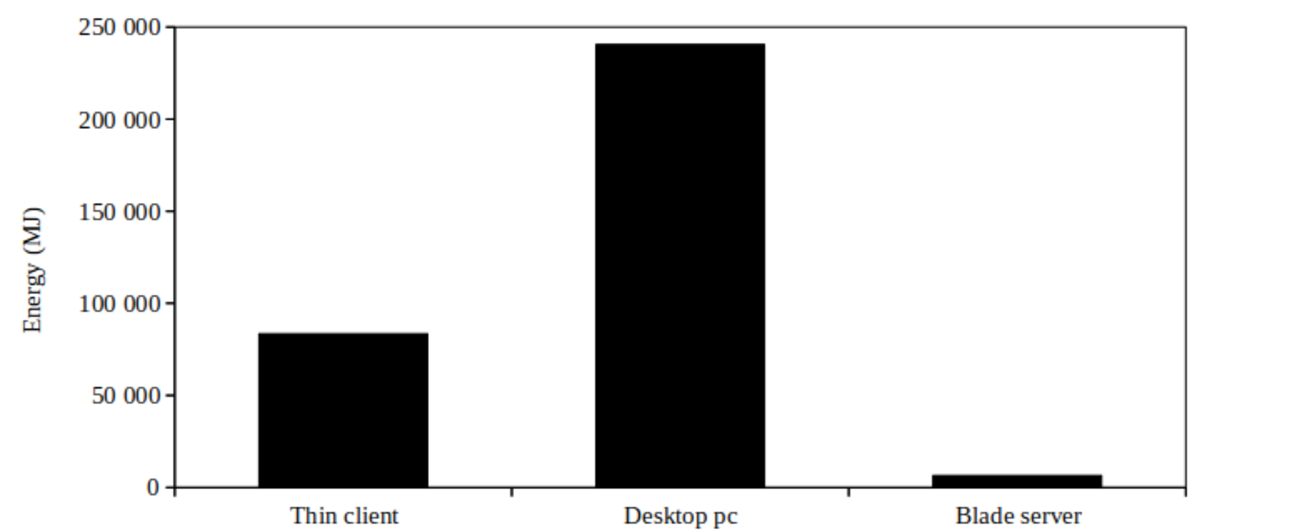
\includegraphics[scale=0.425]{total_energy_use_over_five_years}
  %\end{center}
  \caption{Total energy use of each machine over a five year period.}
  \label{fig:tab1}
\end{figure}

The reference flow has 130 users. Each server provides operations for thirteen
thin
clients. Consequently, the ASP has 130 thin clients and ten servers. The system
of locally hosted software has 130 desktop computers. Multiplying the numbers in
the middle column by the number of machines produces the numbers in the
rightmost column.

\subsection{Life Cycle Impact Assessment (LCIA)}
After acquiring and processing the data, LCAs next have a life cycle impact
assessment (LCIA). For this particular study, the LCIA uses a method called
Eco-Indicator 99. Eco-Indicator 99 has three impact categories: human health,
ecosystem quality, and resource use \cite{pre}. Each impact category has its own
subcategories. For human health, the subcategories include climate
change, ozone layer depletion, carcinogenic effects, respiratory effects, and
ionizing radiation. For ecosystem quality, the subcategories include
ecotoxicity,
acidification, eutrophication, and land use. For resources, the subcategories
include surplus energy from fossil fuels and minerals. 

Alternative impact categories and indicators exist, but they do not serve this
paper's needs as well. This study analyzes the consequences of weighting
different environmental
impacts. Since the tool for assigning weights, the mixing triangle, uses
Eco-Indicator 99, this study's LCA also uses Eco-Indicator 99, including its
impact categories and category indicators \cite{triangle} \cite{pre}.

Eco-Indicator offers three perspectives for characterization. This LCA will use
the individualist perspective because it has a shorter time
perspective than the other two options, the hierarchist and egalitarian
perspectives. According to M. Goedkoop and R. Spriensma in
\textit{The Eco-Indicator 99: A Damage Oriented Method for Life cycle Impact
Assessment}, for the hierarchist and egalitarian
perspectives, the calculations continue until the simulation reaches a steady
state \cite{pre-annex}. This LCA does not need such a long time frame, so it
uses the shorter time horizon assumed buy the individualist perspective.

Each impact category has a characterization model. The individualist
characterization model for human health uses concentrations from emission flows
over a period of 100 to 200 years \cite{pre-annex}. For carcinogenics, the model
only uses
substances that the International Agency for Research on Cancer (IARC) considers
to have sufficient evidence of carcinogenicity. For respiratory emissions, the
characterization varies for each substance, but they all come from calculations
in P. Hofstetter's
\textit{Perspectives in the Life Cycle Impact Assessment: A Structured Approach
to Combine Models of the Technosphere, Ecosphere and Valuesphere} \cite{lcia}.
The global warming information comes from multiple sources by the same author.
The climate change model derives its estimates from General
Circulation Models based scenarios documented in R. Tol's
``Estimates of the damage costs of climate change part 1: Benchmark estimates''
and ``Estimates of the damage costs of climate change part 2: Dynamic
estimates'' \cite{climate1}
\cite{climate2}. The final human health subcategory concern focuses on ozone.
For ozone
layer depletion, the characterization model uses a
hundred year time frame to create equivalency factors as documented in
M. Hauschild's and H. Wenzel's \textit{Environmental Assessment of Products
Volume 2: Scientific Background} \cite{ozone}.

Ecosystem quality has two characterization models relevant to this LCIA. The
first one focuses on ecotoxicity. The European Union System for the Evaluation
of Substances provides a model for the toxicity of each relevant emission, as
documented in T. Vermeire et al.'s article, ``European Union system for the
evaluation of substances (EUSES). Principle and structure''
\cite{euses}. The other model addresses acidification and eutrophication. This
latter model uses the percentage of plants likely to disappear, as calculated on
a
European scale by the Ministry of Housing, Spatial Planning and the Environment
\cite{pre}.

The mechanism by which Eco-Indicator 99 assesses an impact involves taking the
relevant environmental flows and characterizing them as a quantity with a
particular unit. For
example, a few of the processes release carbon dioxide into the environment.
This
carbon dioxide affects human health, so carbon dioxide becomes relevant to the
climate change subcategory and its containing human health impact category.
Every relevant flow has a
characterization factor assigned to it based on the size of its impact. Carbon dioxide has
a characterization factor of 0.013333 $\frac{\textrm{DALY}}{\textrm{kg}}$.
These
characterization factor numbers come from the characterization models for each
impact category.
The researcher multiplies the factor by the
amount of carbon dioxide to
quantify how much it contributed to the category. 

Due to the scale of the task, not every flow in the systems entered into the
assessment. The researcher has to enter every individual flow into
Eco-Indicator from NREL's database, but the large quantity of flows makes
including all of them unrealistic for the time allotted.

\begin{table}[t!]
  \caption{Characterization Factors}
  \label{tab:8}
  %\begin{center}
  \centering
    \begin{tabular}{| l | l | l | l |}
      \hline
      Flow & Subcategory & Category & Impact factor \\
      \hline
      CO$_2$   & Climate change  & HH      & 
        $0.013333 \frac{\textrm{DALY}}{\textrm{kg}}$ \\
      Coal & Fossil fuel     & Resources          &
        $1.0 \frac{\textrm{MJ}}{\textrm{kg}}$ \\
      Dioxins and & Ecotoxicity & EQ & $132000 \frac{\textrm{
        PDF} \cdot \textrm{m}^2 \cdot \textrm{yr}}{\textrm{kg}}$ \\
        \hspace{5mm} furans & & &  \\
      Mercury & Ecotoxicity & EQ & $19.3 \frac{\textrm{PDF} \cdot
        \textrm{m}^2 \cdot \textrm{yr}}{\textrm{kg}}$ \\
      Nickel  & Ecotoxicity & EQ & $90.6 \frac{\textrm{PDF} \cdot
        \textrm{m}^2 \cdot \textrm{yr}}{\textrm{kg}}$ \\
      Nickel  & Carcinogenics & HH &
        $0.00679 \frac{\textrm{DALY}}{\textrm{kg}}$ \\
      Particulates & Respiratory effects      & HH &
        $2.74 \cdot 10^{-4} \frac{\textrm{DALY}}{\textrm{kg}}$ \\
                   & \hspace{5mm} (inorganic) &              &  \\
      SO$_2$ & Acidification and & EQ & $1.041 \frac{
        \textrm{PDF} \cdot \textrm{m}^2 \cdot \textrm{yr}}{\textrm{kg}}$ \\
                     & \hspace{5mm} eutrophication & & \\
      VOC & Respiratory effects & HH &
        $6.0 \cdot 10^{-7} \frac{\textrm{DALY}}{\textrm{kg}}$ \\
          & \hspace{5mm} (organic) & &  \\
      \hline
    \end{tabular}
  %\end{center}
\end{table}

Table \ref{tab:8} shows the characterization factors for the elementary flows
output by the
processes derived from the MEEUP analyses, as well as the elementary flow for
the bituminous coal. For the sake of space, the table uses
the synonymous phrase ``impact factor'' in place of ``characterization factor''
in the table's header. The
researcher fabricated the value for the coal because OpenLCA's
available Eco-Indicator data do
not have any fossil fuel information to use as a point of comparison. The other
values in
the table come from finding equivalent flows in the default Eco-Indicator data.

\subsection{Normalization}
The OpenLCA implementation of Eco-Indicator 99 has
normalization values. The normalization numbers come from a reference value
calculated by the following formula from T. Blonk et al.'s \textit{Drie
Referentieniveau's voor Normalisatie in LCA [Three Reference Levels for
Normalization in LCA]} \cite{blonk} \cite{pre-annex}. 
\begin{equation}
  E_t = P_t \cdot \frac{E_k}{P_K}
\end{equation}
The definition of each symbol follows.
\begin{equation}
  E_t \equiv \textrm{Total emission in Europe}
\end{equation}
\begin{equation}
  P_t \equiv \textrm{Total energy use in Europe}
\end{equation}
\begin{equation}
  E_k \equiv \textrm{Known emission}
\end{equation}
\begin{equation}
  P_k \equiv \textrm{Energy use of countries with known emissions}
\end{equation}

Table \ref{tab:9} summarizes the values that result from this calculation. The
normalization factors come directly from the OpenLCA LCIA database, so this
study uses the same number of significant figures as the database.

\begin{table}[t!]
  \caption{Normalization Factors for Each Impact Category}
  \label{tab:9}
  %\begin{center}
  \centering
    \begin{tabular}{| l | l |}
      \hline
      Impact category   & Normalization factor \\
      \hline
      Ecosystem quality & 5605.3811659 \\
      Human health      & 0.00465332713 \\
      Resources         & 347.46351633 \\
      \hline
    \end{tabular}
  %\end{center}
\end{table}

\subsection{Weighting}
This LCA uses multiple weighting configurations. The configurations compromise
between human health, ecosystem quality, and resource use.
The three weighting factors, one for each impact category, must add up to 100\%.
The researcher multiplies the factors by the corresponding numbers that
represent the impact for one of the categories.
This LCA uses a mixing triangle with the
same impact categories as Eco-Indicator 99, although researchers could
theoretically formulate different categories for weighting \cite{triangle}.

\section{Results and Discussion}
The LCA concludes by presenting the results from the LCIA in raw, normalized,
and weighted forms. Then it moves into an interpretation phase, which
involves identifying issues with the analysis, such as incompleteness of the
data or insufficiency of the impact categories. This Section finishes with
analyzing how the results inform the research questions.

\subsection{LCIA Results}
Tables \ref{tab:10} and \ref{tab:11} show the LCIA results for each system
without weighting. The ASP
has a smaller impact on all three impact categories, so regardless of the
weighting configuration, it will always produce the preferable results in a
comparison between systems. However, the discrepancy between systems might grow
or shrink based on the weights.

\begin{table}[t!]
  \caption{LCIA Results for the ASP}
  \label{tab:10}
  %\begin{center}
  \centering
    \begin{tabular}{| l | l | l |}
      \hline
      Impact category   & Result             & Normalized \\
      \hline
      Ecosystem quality & $1669.12200 \textrm{ PDF} \cdot \textrm{m}^2 \cdot
                          \textrm{yr}$ & $0.29777$ \\
      Human health      & $897.83083$ DALY   & $1.92944 \cdot 10^5$ \\
      Resources & $3.52196 \cdot 10^4$ MJ surplus energy & $101.36191$ \\
      \hline
    \end{tabular}
  %\end{center}
\end{table}
\begin{table}[t!]
  \caption{LCIA Results for the Locally Hosted Software}
  \label{tab:11}
  %\begin{center}
  \centering
    \begin{tabular}{| l | l | l |}
      \hline
      Impact category   & Result             & Normalized \\
      \hline
      Ecosystem quality & $4238.84957 \textrm{ PDF} \cdot \textrm{m}^2
                          \cdot \textrm{yr}$ & $0.75621$ \\
      Human health      & $2289.78568$ DALY   & $4.92075 \cdot 10^5$ \\
      Resources & $9.04187 \cdot 10^4$ MJ surplus energy & $260.22515$ \\
      \hline
    \end{tabular}
  %\end{center}
\end{table}

Table \ref{tab:12} shows the different weighting configurations employed for the
study.
The leftmost column assigns a number to each configuration. These
numbers appear in Tables \ref{tab:13} and \ref{tab:14} and corresponds to the
configurations that appear in Table \ref{tab:12}.

\begin{table}[t!]
  \caption{Weighting Configurations}
  \label{tab:12}
  %\begin{center}
  \centering
    \begin{tabular}{| r | r | r | r |}
      \hline
      Number & Ecosystem quality & Human health & Resources \\
      \hline
      $1$  & $1$    & $0$    & $0$    \\
      $2$  & $0.75$ & $0.25$ & $0$    \\
      $3$  & $0.75$ & $0$    & $0.25$ \\
      $4$  & $0.5$  & $0.5$  & $0$    \\
      $5$  & $0.5$  & $0.25$ & $0.25$ \\
      $6$  & $0.5$  & $0$    & $0.5$  \\
      $7$  & $0.25$ & $0.75$ & $0$    \\
      $8$  & $0.25$ & $0.5$  & $0.25$ \\
      $9$  & $0.25$ & $0.25$ & $0.5$  \\
      $10$ & $0.25$ & $0$    & $0.75$ \\
      $11$ & $0$    & $1$    & $0$    \\
      $12$ & $0$    & $0.75$ & $0.25$ \\
      $13$ & $0$    & $0.5$  & $0.5$  \\
      $14$ & $0$    & $0.25$ & $0.75$ \\
      $15$ & $0$    & $0$    & $1$    \\
      \hline
    \end{tabular}
  %\end{center}
\end{table}

Tables \ref{tab:13} and \ref{tab:14} shows the results after weighting for the ASP and the locally
hosted system, respectively. The rightmost column shows a single score to
evaluate the overall impact of the system. The range of numbers in this column
shows how a weighting configuration can manipulate the outcome of an analysis.

\begin{table}[t!]
  \caption{ASP Results from Various Weighting Configurations}
  \label{tab:13}
  %\begin{center}
  \centering
    \begin{tabular}{| l | l | l | l | l |}
      \hline
      Config. & EQ & HH& Resources & Sum \\
      \hline
      $1$           & $0.29777$   & $0$      & $0$          & $0.29777$ \\
      $2$           & $0.2233275$ & $48\,236$  & $0$          & $48\,236.2233$ \\
      $3$           & $0.2233275$ & $0$      & $25.3404775$ & $25.563805$ \\
      $4$           & $0.148885$  & $96\,472$  & $0$          & $96\,472.14889$ \\
      $5$           & $0.148885$  & $48\,236$  & $25.3404775$ & $48\,261.48936$ \\
      $6$           & $0.148885$  & $0$      & $50.680955$  & $50.82984$ \\
      $7$           & $0.0744425$ & $144\,708$ & $0$          & $144\,708.0744$ \\
      $8$           & $0.0744425$ & $96\,472$  & $25.3404775$ & $96\,497.41492$ \\
      $9$           & $0.0744425$ & $48\,236$  & $50.680955$  & $48\,286.7554$ \\
      $10$          & $0.0744425$ & $0$      & $76.0214325$ & $76.095875$ \\
      $11$          & $0$         & $192\,944$ & $0$          & $192\,944$ \\
      $12$          & $0$         & $144\,708$ & $25.3404775$ & $144\,733.3405$ \\
      $13$          & $0$         & $96\,472$  & $50.680955$  & $96\,522.68096$ \\
      $14$          & $0$         & $48\,236$  & $76.0214325$ & $48\,312.02143$ \\
      $15$          & $0$         & $0$      & $101.36191$  & $101.36191$ \\
      \hline
    \end{tabular}
  %\end{center}
\end{table}
\begin{table}[t!]
  \caption{Results from Various Weighting Configurations for the Locally Hosted
           System}
  \label{tab:14}
  %\begin{center}
  \centering
    \begin{tabular}{| l | l | l | l | l |}
      \hline
      Config. & EQ & HH & Resources & Sum \\
      \hline
      $1$  & $0.75621$   & $0$          & $0$           & $0.75621$ \\
      $2$  & $0.5671575$ & $123\,018.75$  & $0$           & $123\,019.3172$ \\
      $3$  & $0.5671575$ & $0$          & $65.0562875$  & $65.623445$ \\
      $4$  & $0.378105$  & $246\,037.5$   & $0$           & $246\,037.8781$ \\
      $5$  & $0.378105$  & $123\,018.75$  & $65.0562875$  & $123\,084.1844$ \\
      $6$  & $0.378105$  & $0$          & $130.112575$  & $130.49068$ \\
      $7$  & $0.1890525$ & $369\,056.25$  & $0$           & $369\,056.4391$ \\
      $8$  & $0.1890525$ & $246\,037.5$   & $65.0562875$  & $246\,102.7453$ \\
      $9$  & $0.1890525$ & $123\,018.75$  & $130.112575$  & $123\,149.0516$ \\
      $10$ & $0.1890525$ & $0$          & $195.1688625$ & $195.357915$ \\
      $11$ & $0$         & $492\,075$     & $0$           & $492\,075$ \\
      $12$ & $0$         & $369\,056.25$  & $65.0562875$  & $369\,121.3063$ \\
      $13$ & $0$         & $246\,037.5$   & $130.112575$  & $246\,167.6126$ \\
      $14$ & $0$         & $123\,018.75$  & $195.1688625$ & $123\,213.9189$ \\
      $15$ & $0$         & $0$          & $260.22515$   & $260.22515$ \\
      \hline
    \end{tabular}
  %\end{center}
\end{table}

\subsection{Discussion}
Table \ref{tab:15} shows the difference between the sums of the two systems at
each
weighting configuration. It presents the data sorted by the difference. The more
weight assigned to human health, the greater the discrepancy. Resource use
follows human health in terms of producing the largest difference, and
configurations that place more weight on ecosystem quality produce the smallest
differences.

\begin{table}[t!]
  \caption{Difference between the Sums of the Two Systems}
  \label{tab:15}
  %\begin{center}
  \centering
    \begin{tabular}{| r | r | r | r |}
      \hline
      Ecosystem quality & Human health & Resources & Difference \\
      \hline
      $0$               & $1$          & $0$       & $299\,131$ \\
      $0$               & $0.75$       & $0.25$    & $224\,387.9658$ \\
      $0.25$            & $0.75$       & $0$       & $224\,348.3647$ \\
      $0$               & $0.5$        & $0.5$     & $149\,644.9316$ \\
      $0.25$            & $0.5$        & $0.25$    & $149\,605.3304$ \\
      $0.5$             & $0.5$        & $0$       & $149\,565.7292$ \\
      $0$               & $0.25$       & $0.75$    & $74\,901.89747$ \\
      $0.25$            & $0.25$       & $0.5$     & $74\,862.2962$ \\
      $0.5$             & $0.25$       & $0.25$    & $74\,822.69504$ \\
      $0.75$            & $0.25$       & $0$       & $74\,782.5267$ \\
      $0$               & $0$          & $1$       & $158.86324$ \\
      $0.25$            & $0$          & $0.75$    & $119.26204$ \\
      $0.5$             & $0$          & $0.5$     & $79.66084$ \\
      $0.75$            & $0$          & $0.25$    & $40.05964$ \\
      $1$               & $0$          & $0$       & $0.45844$ \\
      \hline
    \end{tabular}
  %\end{center}
\end{table}

Fig. \ref{fig:tab2} shows a graph of the sums for each system for every
configuration. The ASP never generates a higher number, suggesting that the ASP
invariably has a smaller impact. A few of the graph's bars do not show up
because
of their small size. The bars that are too small to show up in the graph come
from configurations that do not emphasize human health.

\begin{figure}[t!]
  %\begin{center}
  \centering
    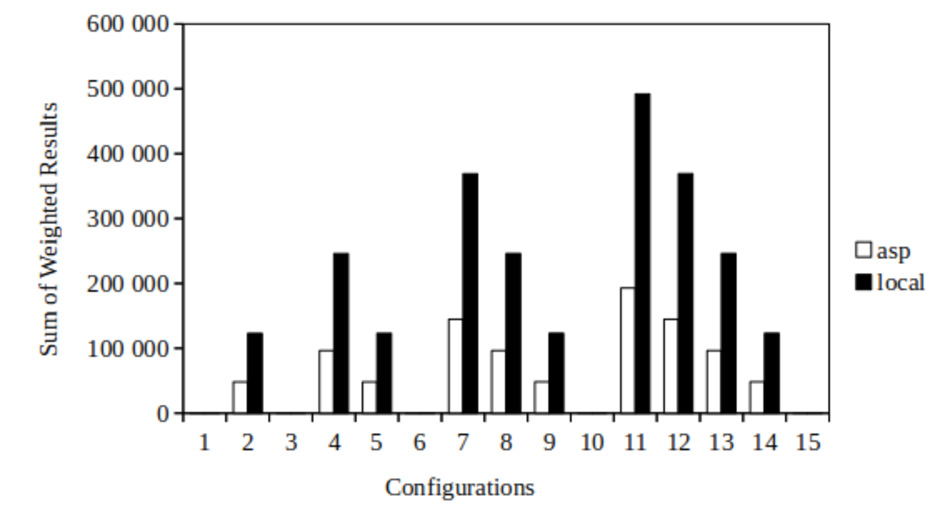
\includegraphics[scale=0.55]{sums}
  %\end{center}
  \caption{The sums of each system.}
  \label{fig:tab2}
\end{figure}

One interpretation of the data suggests that an environmental analysis that
places little concern on human health would show little reason to
pick one design over the other. However, the differences between the sums
correlate with the
overall size of the effects. In other words, the increase in the difference
between overall effects
reflects an increase in the size of the overall effect. Tables \ref{tab:13}
and \ref{tab:14} show
that human health produces larger numbers for both systems. The dominance of
human health comes from the carbon dioxide, which makes up over 99\% of the
human health effects for both systems. These results suggest that
designers should focus almost exclusively on global warming potential because
the other impacts have such a small effect unless the weighting for human
health approaches zero.

Ultimately, the results do not offer a clear answer to how a weighting
configuration might
dictate system design. They suggest that a centralized system offer
a superior option to a decentralized system. However, the approximations on the
systems favor the centralized design. The absence of networking equipment in the
LCA may cause an underestimation of the ASP's impact. Also, the results suggest
that energy use correlates with raw material use. The ASP does not have as much
physical material, and it correlatingly uses less energy.

Fig. \ref{fig:tab3} and Fig. \ref{fig:tab4} present a graphical comparison of the
energy and mass of the two systems. The two features correlate. The system with
more mass uses more energy present a graphical comparison of the energy and mass
of the two systems. The two features correlate. The system with more mass uses
more energy.

For the first research question, the results indicate that the weighting
configurations have a negligible effect on design decisions because the results
uniformly favor the centralized deign. If one of the configurations had produced
numbers showing a smaller impact for the decentralized method, then the results
would have shown the significance of weighting. This event did not occur, so
nothing in the study shows that weighting configurations will affect design very
much. However, the results of this study may not generalize to other systems, so
the reader should not take this answer as proof that weighting does not affect
design.

For the second research question, the results suggest that environmental
consequences
correlate. Tables \ref{tab:13} and \ref{tab:14} show that the locally hosted
system has
an impact at least as large as the ASP in every impact category. However, as
with the answer to the first research question, the
reader should take caution in generalizing this result to other systems.

\begin{figure}[t!]
  %\begin{center}
  \centering
    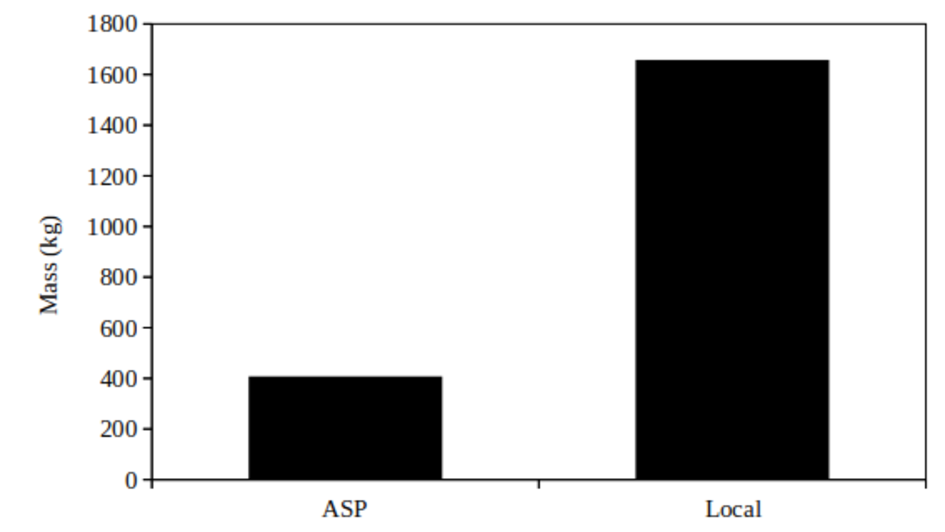
\includegraphics[scale=0.55]{mass}
  %\end{center}
  \caption{The mass of each system.}
  \label{fig:tab3}
\end{figure}
\begin{figure}[t]
  %\begin{center}
  \centering
    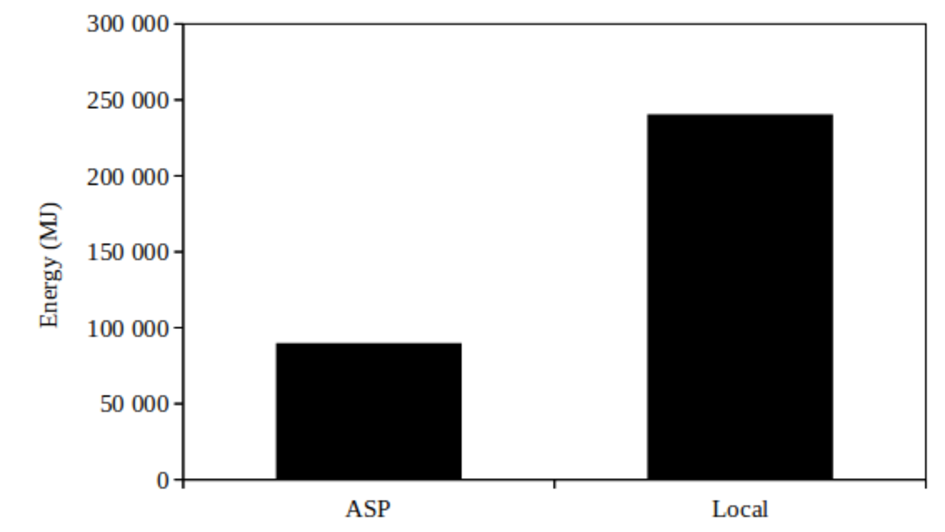
\includegraphics[scale=0.55]{energy}
  %\end{center}
  \caption{The energy of each system.}
  \label{fig:tab4}
\end{figure}

\subsection{Analytical Investigation}

\section{Conclusion}
The study found that the weighting did not change which
of the two system designs has a smaller overall environmental impact. It also
found
that the different types of impacts correlate with the systems tested, making
weighting negligible.

\subsection{Concluding Positions}
The results suggest similar conclusions as past studies, thereby confirming and
strengthening their evidence. These past results
concluded that server client
models have a smaller environmental impact than equivalent systems that run on
desktop computers. This study produces no evidence of tradeoffs for this type
of system. However, these results might not generalize to centralized and
decentralized systems. This paper focuses on centralization
in a hardware sense. For software, centralized systems might not
always have a smaller impact. For example, the operating systems that manage
servers often have decentralized structures, and this study found lower impacts
with server-based systems.

The impact factors had a much greater effect on the results than the weighting.
The only time the human health impact category did not dominate occurred when
the researcher set its weight to zero. The biggest emission contribution comes
from carbon dioxide equivalents. This result suggests that global warming
causes significantly more damage than any other environmental consequence
included in the Eco-Indicator data. Because of the dominance of this impact
category, weighting has a minimal effect.

\subsection{Implications}
The results imply that the established wisdom of green technology design is
valid. Nothing in the results indicates a problem with the conclusions of
past research. The issue with making tradeoffs among impacts comes from the
potential of creating disastrous consequences in one category to improve the
situation in another. However, the lack of tradeoffs found in this study
immunizes the examined systems to this problem. System designers do not
always have to compromise among impacts.

The results also imply that global warming is the most significant consequence
with respect to these systems. Assuming the accuracy of the  characterization
factors in Eco-Indicator 99, the other impacts have relatively little effect.
The results suggest that computer systems contribute to global warming potential
more than any other category. Because of the magnitude of this category, system
designers do not need to use an all-inclusive approach such as the LCA to
gauge the impact of their designs. A less demanding alternative that focuses
exclusively on carbon emissions will suffice.

\subsection{Limitations}
This study has numerous limitations. Data availability severely restricts how
the LCA progresses. The lack of information completely dictates both the system
boundary and data requirements. The databases contain errors, and portions of
their
contents comes from over a decade ago. The study does not account for all the
hardware components. For computer monitors, this detail does not matter because
both systems theoretically have the same number and type of monitors. But for
network hardware, an issue arises because the ASP needs more networking material
than its alternative. Finally, the data assume all energy comes from bituminous
coal in the form of electricity.

\subsection{Future Research}
Future research can further investigate how the methodologies behind impact
assessment affect designs. Other systems, especially those that involve
compromises among impact categories, would produce different results when
tested with multiple weighting configurations. Other future research might
entail performing LCAs on smaller products. Components from smaller product
systems build up larger, complex systems in the LCA method, so having a
catalogue of research on individual parts would enable researchers to conduct
assessments more easily and accurately. Finally, future research can focus on
how less demanding assessment methods differ in their results from their
more expansive counterparts. LCA demands rigor, so if
it does not add much beyond what a less-rigorous method would find,
engineers and analysts might know when to avoid it.





% if have a single appendix:
%\appendix[Proof of the Zonklar Equations]
% or
%\appendix  % for no appendix heading
% do not use \section anymore after \appendix, only \section*
% is possibly needed

% use appendices with more than one appendix
% then use \section to start each appendix
% you must declare a \section before using any
% \subsection or using \label (\appendices by itself
% starts a section numbered zero.)
%


%\appendices
%\section{Proof of the First Zonklar Equation}
%Appendix one text goes here.

% you can choose not to have a title for an appendix
% if you want by leaving the argument blank
%\section{}
%Appendix two text goes here.

%Balance the columns of the final page
%\enlargethispage{-0.631in}

% use section* for acknowledgment
\section*{Acknowledgment}


The authors thank Prof. Michael Hoffman and Prof. Reza Toossi
of CSU Long Beach for their feedback.


% Can use something like this to put references on a page
% by themselves when using endfloat and the captionsoff option.
\ifCLASSOPTIONcaptionsoff
  \newpage
\fi



% trigger a \newpage just before the given reference
% number - used to balance the columns on the last page
% adjust value as needed - may need to be readjusted if
% the document is modified later
%\IEEEtriggeratref{8}
% The "triggered" command can be changed if desired:
%\IEEEtriggercmd{\enlargethispage{-5in}}

% references section

% can use a bibliography generated by BibTeX as a .bbl file
% BibTeX documentation can be easily obtained at:
% http://mirror.ctan.org/biblio/bibtex/contrib/doc/
% The IEEEtran BibTeX style support page is at:
% http://www.michaelshell.org/tex/ieeetran/bibtex/
%\bibliographystyle{IEEEtran}
% argument is your BibTeX string definitions and bibliography database(s)
%\bibliography{IEEEabrv,../bib/paper}
%
% <OR> manually copy in the resultant .bbl file
% set second argument of \begin to the number of references
% (used to reserve space for the reference number labels box)
%%\begin{thebibliography}{11}

\bibliographystyle{myIEEEtran}
\bibliography{references,IEEEabrv}

% biography section
% 
% If you have an EPS/PDF photo (graphicx package needed) extra braces are
% needed around the contents of the optional argument to biography to prevent
% the LaTeX parser from getting confused when it sees the complicated
% \includegraphics command within an optional argument. (You could create
% your own custom macro containing the \includegraphics command to make things
% simpler here.)
%\begin{IEEEbiography}[{\includegraphics[width=1in,height=1.25in,clip,keepaspectratio]{mshell}}]{Michael Shell}
% or if you just want to reserve a space for a photo:

\begin{IEEEbiography}[{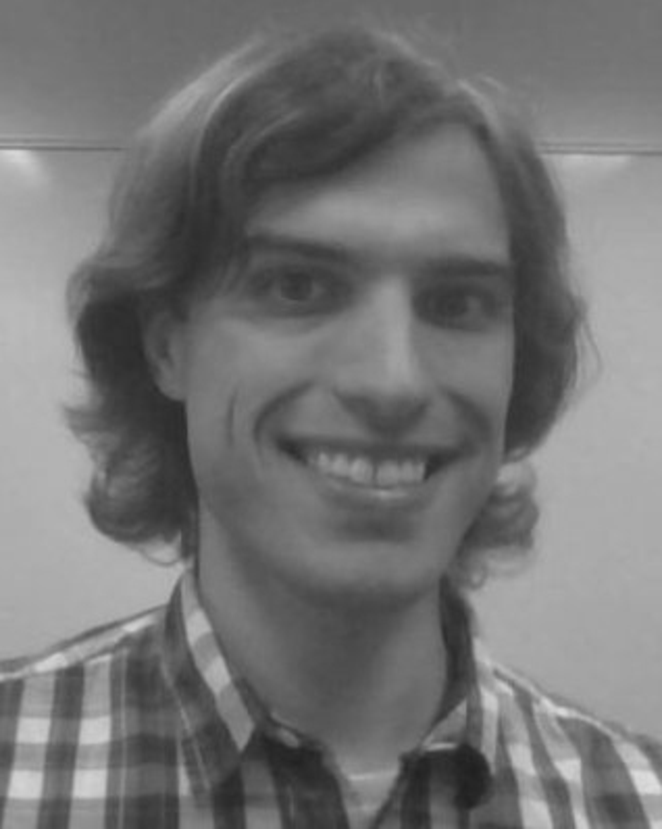
\includegraphics[width=1in,height=1.25in,clip,%
%keepaspectratio
]{bert}}]{Bertrand Ithurburn}
(M'15) received the BS degree in computer science and engineering from the
University of California, Davis, CA, USA in 2014 and the MS degree in computer
science from California State University, Long Beach, CA, USA in 2016. He is
graduate student at the Graduate Center at City University of New York, NY, USA.
\end{IEEEbiography}

\begin{IEEEbiography}[{
\includegraphics[width=1in,height=1.25in,clip,%
%keepaspectratio
]{penzenstadler}}]{Birgit Penzenstadler}
(M) received the PhD degree from the
Technical University of Munich, Germany in 2011.

She is an Assistant Professor of software engineering at California State
University, Long Beach. Her research focuses on software engineering for
sustainability and resilience, and she leads the Resilience Lab at CSULB.
\end{IEEEbiography}

%\begin{IEEEbiographynophoto}{Bertrand Ithurburn}
%\end{IEEEbiographynophoto}

% You can push biographies down or up by placing
% a \vfill before or after them. The appropriate
% use of \vfill depends on what kind of text is
% on the last page and whether or not the columns
% are being equalized.

%\vfill

% Can be used to pull up biographies so that the bottom of the last one
% is flush with the other column.
%\enlargethispage{-5in}



% that's all folks
\end{document}


